\documentclass{ieeeaccess}
\usepackage{cite}
\usepackage{amsmath,amssymb,amsfonts}
\usepackage{algorithm}
\usepackage{algorithmicx}
\usepackage{algpseudocode}
\usepackage{graphicx}
\usepackage{textcomp}

\ifCLASSOPTIONcompsoc
\usepackage[caption=false, font=normalsize, labelfont=sf, textfont=sf]{subfig}
\else
\usepackage[caption=false, font=footnotesize]{subfig}
\fi

\ifCLASSINFOpdf
   \usepackage{graphicx}
   \usepackage{lipsum}
   \usepackage{booktabs}
   \usepackage{threeparttable}
   \usepackage{caption}
   \usepackage{epstopdf}
   \usepackage{cite}
\else
\fi

\usepackage{xcolor}

\def\BibTeX{{\rm B\kern-.05em{\sc i\kern-.025em b}\kern-.08em
    T\kern-.1667em\lower.7ex\hbox{E}\kern-.125emX}}
\begin{document}
\history{Date of publication xxxx 00, 0000, date of current version xxxx 00, 0000.}
\doi{10.1109/ACCESS.2017.DOI-}

\title{Unfolding the City: Spatial Preference Based on Individual Demographic Characteristics}


\author{\uppercase{Qi wang}\authorrefmark{1,2}, \uppercase{min lu}\authorrefmark{2,3} and \uppercase{Qingquan Li}\authorrefmark{1,2}}
\address[1]{State Key Laboratory of Information Engineering in Surveying, Mapping and Remote Sensing, Wuhan University, Wuhan 430072, China}
\address[2]{Shenzhen Key Laboratory of Spatial Smart Sensing and Services, Shenzhen University, Shenzhen 518060, China}
\address[3]{School of Architecture and Urban Planning, Shenzhen University, Shenzhen 518060, China}

\tfootnote{This work was jointly supported by the National Natural Science Foundation of China(No. 71961137003 and No. 41671387).}


\markboth
{Author \headeretal: Preparation of Papers for IEEE TRANSACTIONS and JOURNALS}
{Author \headeretal: Preparation of Papers for IEEE TRANSACTIONS and JOURNALS}

\corresp{Corresponding author: Qingquan Li (e-mail: liqq@szu.edu.cn).}

\begin{abstract}
A city is shaped not only by its assembled infrastructures but also by the people living inside it. People with a wide range of individual demographic characteristics visit places at different weights and with different preferences, sculpting a city into a space of diverse spatial preferences. Compared with the well-studied anonymous travel behaviors, the daily movement of characterized individuals has been less studied due to the challenges in the collection and analysis of data considering privacy. In this work, we take a step forward and perform an online census to collect individual profiles and movements from volunteers on a large-scale. Then, we design a visual analytic system to investigate the spatial preferences of groups by specifying demographic characteristics. To facilitate the identification of characterized groups, individuals are embedded in t-SNE projection for an abstract overview, and vivid graphics are drawn by a data-driven profile method for detailed examination. A 2.5D spatial visualization is proposed to maintain a compact multivariable analysis by relaxing the z-axis to encode information, such as visiting frequency, demands, and traveling distance. Together with a cross-filter and flexible 2.5D interactions, the effectiveness and usability of the system are demonstrated well by a study conducted in Shenzhen.\end{abstract}

\begin{keywords}
Visual analytics, spatial preference, individual characteristics, data collection
\end{keywords}

\titlepgskip=-15pt

\maketitle

\section{Introduction}
\label{sec:introduction}
\PARstart{T}{he} science fiction novella \textit{Folding Beijing}~\cite{hao2016_foldingbeijing} depicts a world where three social classes of people live in independent spatiotemporal patterns, though sharing the same earth surface. This work is an artistic metaphor for one possibility that people prefer to select different places to live according to their individual characteristics, especially their personal demographic characteristics. This phenomenon has attracted research interest for a long time in the sociological field. In 1970, Pahl~\cite{pahl1975whose} posed the question "whose city" and expressed interest in understanding territorial inequalities. Contemporary contestation also continually raises the banner "The City Belongs to All!"~\cite{Mayer2017_whosecity}. Some approaches include discussing spatial distribution~\cite{RN909}, spatial interaction~\cite{RN1692} and place attractiveness~\cite{retailcity}. However, because of the lack of movement characteristics, these aspects were analyzed from a spatial perspective, and individual characteristic factors were not placed into the context of the problems. It is necessary to explore the relationship between spatial preference and individual demographic characteristics for better region utilization, greater diversity, and opportunity promotion.

Due to the multidimensional nature of demographic characteristics and the spatial diversity of movements, it is challenging to explore, analyze and express the relationship between these parameters. In recent decades, the power of visual analytics in urban problems has been recognized and developed well~\cite{wang2013visual, zeng2013visualizing}. The presence of social media applications fuels spatial analysis with rich semantic texts, so researchers can explore the thematic meaning of the movement behaviors, such as events~\cite{chen2017map} and topics~\cite{bosch2013scatterblogs2}. These works essentially contribute to deepening the contextual understanding of movement activities.  Some works dive deep and infer individual characteristics from social media profiles~\cite{peddinti2014internet} to better describe the semantics of movement behavior. However, due to the limited exposure of personal information, there is still a research gap between understanding the movement behavior and underlying characteristics of movers.
%The question of how to intuitively discover the relationship between spatial preference and multidimensional characteristics is worthy of further investigation.


In this work, we aim to probe deeper in this direction and contextualize the analysis of citizens' spatial preferences against the backdrop of individual demographic characteristics. With this motivation, we ran a campaign to obtain the demographic characteristics of individuals and their daily movements. Conventional offline census requires too much effort and time. With the wide use of mobile devices, we collected information online; we released an online data sourcing program on a social media application that collected data for over half a year. The demographics and movement information of over 10K volunteers were collected during this period. Based on the data collected, we developed a visual analytics system to explore the association between spatial preference and individual demographic characteristics. The system incorporates visualizations of individuals' characteristics, including t-SNE for an overview and data-driven profile visualization for a detailed analysis, as well as 2.5D spatial visualization to explore the spatial distribution of movements. Finally, applying our method in Shenzhen, we derived several cases to demonstrate the power of our method. This work makes two contributions:

(1) We investigate spatial preference with individual demographic characteristics, which is a natural step in research on understanding the social behaviors of a city.

(2) We develop a visual analytic system, whose effectiveness and usability are demonstrated well by a study conducted in Shenzhen.



\section{Related Work}
This work concerns the research topic on visual analytics of movement data and the movers. Many related works focus on the spatiotemporal analysis of movement data in the absence of thematic information. The presence of geotagged social media data facilitates the exploration of thematic information along with movement information. Therefore, the related work is discussed from two aspects: movement data analysis, and geo-tagged social media data analysis.

\subsection{Movement data analysis}
With the development of location-acquisition techniques, massive spatial trajectories are collected to keep track of the trajectories of various moving objects. Techniques have been proposed to process and mine trajectories for spatial knowledge~\cite{Zheng2015_trajectory}. In the field of visualization and visual analytics, spatial visualizations are specifically designed for time, location, spatiotemporal information and other properties in movement data~\cite{chen2015survey}. Wang et al.~\cite{wang2013visual} extract traffic jam propagation graphs to reveal underlying data patterns. Guo et al.~\cite{guo2011tripvista} and Zeng et al.~\cite{zeng2013visualizing} construct geographic regions and visually aggregate the in-between movements as flows. To discover route travel patterns, Lu et al.~\cite{lu2015trajrank} propose TrajRank to explore route travel behavior based on ranking. For multiple routes, Liu et al.~\cite{liu2011_routediversity} study the route diversity between locations and Lu et al.~\cite{Lu2017_multipleroute} explore the route choice behavior among multiple routes. These large number of visual analytics tools and applications cover situation-aware exploration, pattern discovery and traffic situation monitoring. However, they prefer to discuss spatial feature of movements, neglecting the characteristics of the movers and the relationship between movement and movers. In this work, we focus on this to explore how to design visual analytics methods to relate demographic characteristics to spatial feature of movements.


\subsection{Geo-tagged Social Media Data Analysis}
In the presence of social media services, social media data with geo-tags are collected to track people's movements in their daily lives. As an analog of remote sensing data in social science research, geospatial big data has been proposed as social sensing ~\cite{liu2015social}. Hence, analyzing movement information along with rich text has become a popular research area in recent years. Krueger et al.~\cite{krueger2014visual} uses GPS and location-based service data to support the analysis of movement behaviors. Cao et al.~\cite{cao2012whisper} proposes \textit{Whisper} for tracing the pathways of tweets along a spatial hierarchical layout to investigate how information flows among multiple places. Some other researchers tend to infer real information, such as names, gender, and race, from social media data to form the image of social media users based on the demographic characteristics~\cite{peddinti2014internet} and analysis the impact of characteristics on urban human mobility patterns~\cite{luo2016explore}. These works infer thematic information from semantic texts. By analyzing the texts, these works explain what drives movement activities or what results from these activities. This work continues thematic research on movement data but focuses more on individual demographic characteristics. Since real information is not enforced in social media, incorrect inference is inevitable. The biases inherent in social media usage need to be assessed in social research and the deployment of social media data need to be evaluated in research applications~\cite{Longley2015, Paul2016_twitter} . Therefore, based on a census experiment, this work is able to analyze profile information directly to eliminate indirect data inferred from social media data as other related works do. Then an intuitive visualization is proposed to describe these characteristics of individuals.
\section{motivation}

\label{sec:concept}
This work was inspired in a meeting with two domain experts who work on human mobility and urban informatics in the geospatial field. The experts pointed out that as big and open data has evolved, the scope of urban research has been lifted from the spatial perspective up to the social-spatial perspective. There is increasing research interest in understanding how categories of citizens with certain demographic characteristics visit places during their daily lives. Do people select places according to preferences that are intrinsically affected by their socioeconomic characteristics? Is there a limitation to or probability of interaction between different socioeconomic groups in public spaces? With the advances in data acquisition and analysis techniques, these experts demanded to go beyond the conventional static sampled questionnaires, that usually survey visiting preferences. They sought to reveal the spatial distribution in real-world visiting logs and urged for the creation of a dynamic system that supports the interactive exploration of spatial preference in different contexts of demographic characteristics.

Thereafter, we began this project with several rounds of discussions to frame the research problem with two core contents and a research procedure. The first content is \textbf{demographic characteristics}. The demographic characteristics of a person or a group of individuals are the descriptors that contribute to the specifications of populations. This work intends to cover these characteristics from multiple facets, including descriptors such as gender, income, and education. The second content is \textbf{spatial preference}. This content is reflected by the popularity of a place for visiting.

Motivated by their research interest of the experts to understand the spatial preference with individual demographic characteristics, we go through a procedure consisting of two stages, i.e., data collection and basic reviewing and visual analytics design iteration with expert feedback.

\section{Data Description}
\label{subsec:pipeline}
Considering that no existing public dataset can fit our topic well, this work is consolidated with self-maintained data sourcing. We release an online information survey to collect the demographic characteristics and movement logs of individuals over almost half a year. Then a series of statistical analyses are performed on the collected data for sampling bias checking.

\subsection{Online Survey}

The advent of mobile sensing techniques and social media applications makes it possible to collect spatial data through apps within phones. Complementary to the conventional survey, this method is convenient, does not take much manpower and provides precise spatial locations by GPS instead of semantic descriptions.

In this work, we perform a survey in Shenzhen, which is one of the most modern metropolises in China. The experiment is deployed on WeChat, the most widely used social media mobile application in China. Fig. \ref{fig:app} shows the interfaces of the survey app. For privacy issues, all the detailed personal information is desensitized to categorical levels. Considering the main aim of the relationship between spatial preference and demographic characteristics, two crucial aspects need to be collected:

\textbf{Demographic Characteristics} Fig. \ref{fig:data_over} lists the eight domains needed to give a generalized description of an individual. The profile serves as the components for the analysis of mobility patterns of diverse individuals.

\textbf{Traveling Trips} Individuals can upload dynamic traveling trips (Fig. \ref{fig:app}(b)). Each trip requires information on the start/end location, start/end time, traveling purpose, and traveling mode. Locations are recorded by GPS modules in the phones. To encourage trip uploading, a credit system retains the contribution of individuals on trips and rewards the volunteers with the top credits (Fig. \ref{fig:app}(c)).


\begin{figure}
 \centering
 \includegraphics[width=9cm]{pictures/survey_app_eng}
  \captionsetup{justification=centering}
 \caption{Census app interface: (a) personal characteristics collection page; (b) trips collecting page; and (c) credit system page. (In the real census survey, the contents are shown in Chinese.)}
 \label{fig:app}
\end{figure}


\begin{figure}
 \centering
 \includegraphics[width=9cm]{pictures/data_over}
 \captionsetup{justification=centering}
 \caption{Profile of Individual: eight individual characteristics that enrich the analysis of spatial preference.}
 \label{fig:data_over}
\end{figure}



\subsection{Statistics of Collected Data}

Over the release time period from 2015-11 to 2016-01, 21,435 individuals participated in the census, and 229,155 trips were collected.

Our case-study data are confined to a small proportion of WeChat users who opt to contribute their demographic profiles and movements. Considering the caveat that self-selecting individuals are unlikely to represent any clearly defined population~\cite{Longley2015}, we calculate a series of preliminary statistics. In Fig. \ref{fig:data_overview}, the population distribution of each characteristic is shown. The length of the block is coded for population quantity.

\begin{figure}[htb!]
 \centering % avoid the use of \begin{center}...\end{center} and use \centering instead (more compact)
 \includegraphics[width=\columnwidth]{pictures/data_overview}
 \caption{Preliminary statistics of each characteristic in collected demographic data.}
 \label{fig:data_overview}
\end{figure}


The figure shows that, 51.2\% of the participating citizens are male and 48.8\% are female. This result is consistent with governmental statistics stating that 47\% of all citizens are female and 53\% are male\footnote{http://tjj.sz.gov.cn/zwgk/zfxxgkml/tjsj/tjgb/201804/t20180427\_11800902.htm}. The age collected covers a wide range, with ages between 18 and 45 dominating. There are also records pertaining to individuals below the age of 18 or above 70. According to the 2015 Annual Census Statistics report\footnote{http://www.sztj.gov.cn/xxgk/tjsj/pcgb/201606/t20160614\_3697000.htm}, people aged 15-64 comprise 83.23\%, and the median age is 31.5. The age distribution in the collected data aligns with the fact that Shenzhen is a city where the majority of the population is young. From the distribution of education levels, ranging from low to high, technical colleges and universities dominate the samples at a 61\% occupancy rate. The majority get paid less than 200,000. Citizens with higher salaries are also reached in our census. Due to the lack of governmental statistics, we cannot verify that all the characteristics collected are consistent with all the citizens in Shenzhen. From the perspective of surveys, there is always inevitable bias inherent in fully representing the ground truth of the population. However, the preliminary statistical analysis shows the rich scope of the data, which is positive evidence of a relatively even sampling of the population of the city.


\iffalse
Fig. \ref{fig:data_age_edu} gives the distribution of gender, age and education over the population. For participated citizens, 48\% of them are female and 52\% are male. It is consistent with governmental statistics that 47\% of the whole citizens are female and 53\% are male\footnote{http://tjj.sz.gov.cn/zwgk/zfxxgkml/tjsj/tjgb/201804/t20180427\_11800902.htm}. The age collected covers a wide range, dominating between 18 and 45. There are also records pertaining to individuals below the age of 18 or above 70. According to the 2015 Annual Census Statistics report\footnote{http://www.sztj.gov.cn/xxgk/tjsj/pcgb/201606/t20160614\_3697000.htm}, people aging 15-64 occupy 83.23\% and the median age is 31.5. The age distribution in collected data follows the fact that Shenzhen is a city where the majority is young. Fig, \ref{fig:data_age_edu}(b) gives the distribution of education levels, ranging from low to high. The technical college and university dominate the samples at the 61\% occupancy rate. Fig. \ref{fig:data_job_inc}(a) shows the job types of sampled individuals, who are servants, workers, officers, businessmen and so on. \colorbox{yellow}{Fig. \ref{fig:data_job_inc}(b) gives the radar diagram of the annual pay.} The majority get paid below 200,000. Citizens with higher salary are also reached in our census.

\begin{figure}[htb!]
 \centering % avoid the use of \begin{center}...\end{center} and use \centering instead (more compact)
 \includegraphics[width=\columnwidth]{pictures/data1}
 \caption{Age and Education Distribution: (a) age; (b) education.}
 \label{fig:data_age_edu}
\end{figure}


\begin{figure}[htb!]
 \centering % avoid the use of \begin{center}...\end{center} and use \centering instead (more compact)
 \includegraphics[width=\columnwidth]{pictures/data2}
 \caption{Job and Income Distribution: (a) job; (b) income}
 \label{fig:data_job_inc}
\end{figure}
\fi

The basic statistics related to movements are shown in Fig. \ref{fig:data_geometry}. Fig. ~\ref{fig:data_geometry}(a) visualizes the distribution of the trip quantity of each citizen. The distribution has a heavy-tail, which follows the trends of most human-related statistics. In Fig. ~\ref{fig:data_geometry}(b), the active traveling time (here, we take the start time as representative of the active time) follows the common knowledge about urban life. There are obvious morning and evening rush hours. Fig. ~\ref{fig:data_geometry}(c) shows the counts for different traveling purposes. Ninety-five percent of trips are tagged with a clear traveling purpose in the data. Thirty-three percent of trips are going home, and 37\% are going to work. In addition to this kind of routine travel, there are also substantial numbers of trips for other purposes such as going shopping and going the hospital. Fig. ~\ref{fig:data_geometry}(d) shows the spatial distribution of the origins and destinations. It is found that more dots are located in Futian and Nanshan Districts, the city's heart, than in the surrounding areas. This result is consistent with Batty's exposition of the focus of city networks and interaction patterns~\cite{batty2013new}.


\begin{figure}[htb!]
 \centering % avoid the use of \begin{center}...\end{center} and use \centering instead (more compact)
 \includegraphics[width=\columnwidth]{pictures/data3_2}
 \caption{Statistics of trips: (a) distribution of trip quantities for each citizen; (b) start time of trips; (c) purpose of trips; and (d) distribution of origins/destinations. }
 \label{fig:data_geometry}
\end{figure}



\section{Visual Design}

The design of the visual analytics system is iterated via multipass discussions with the two domain experts. In this section, we first introduce specific tasks that the system is intended for and the design rationales aligned to provide a user-friendly interface for domain experts. Then, we introduce the visual design.

\subsection{Tasks}

The exploration of core contents (introduced in Section~\ref{sec:concept}) is resolved further with the following tasks.

\begin{itemize}
\item \textbf{Task 1: Identify groups with specific individual demographic characteristics}: to obtain groups of people with common or similar attributes and to explore the correlation among individual characteristics.
\item \textbf{Task 2: Explore the spatial preference of a group}: to explore where, how and why the group of interest moves in the city.
\item \textbf{Task 3: Compare spatial preference among multiple groups}: to express the similarities and differences between different groups in their spatial preferences and to investigate the relationship between movement and individual demographic characteristics.
\end{itemize}

\begin{figure*}[htb!]
 \centering
 \includegraphics[width=18.1cm]{pictures/teaser.eps}
 \caption{System Interface: (a) an interactive infographics provides the basic statistical facets of individuals; (b) a t-SNE visualization gives an overview of individuals, where the similarity in high-dimensional space is preserved in 2D space; (c) data-driven profiles support users with organic individual perception; (d) a group of individuals of interest can be saved; (e) the movement of the chosen group is visualized and explored in the 2.5D main view; (f) a dock is provided to restore and compare findings; and (g) different choices of 2.5D encoding can be selected.}
 \label{fig:teaser}
\end{figure*}

\subsection{Design Considerations}

With the three tasks above, we derive the following design considerations:

\begin{itemize}
\item \textbf{Intuitive perception of an individual as an organic complex (C1)}: the system should make use of end-user daily experience in sensing individual demographic characteristics to provide intuitive visualization instead of lifeless representation by numbers. The visual design needs to help end-users to pick desirable information from the whole.
\item \textbf{Good overview of multivariate individuals (C2)}: following the visual analytics mantra of Shneiderman~\cite{RN459}, it is very important to provide a good overview of all the individuals so the users know where to explore.
\item \textbf{Effective multivariable cross-filter for individual characteristics (C3)}: there are eight domains for describing an individual. The system is supposed to provide a straightforward method for easy filtering by the eight criteria.
\item \textbf{Compact visualization of spatial preference in the constraint of spatial space (C4)}: the analysis of spatial preference not only includes the conventional spatial and temporal dimensions but also other abstract dimensions, e.g., travel purpose and visiting frequency. The system should have a compact layout to support simple correlation between spatial and abstract information.
\item \textbf{Flexible interactions for exploring spatial preference either within one group or between groups (C5)}: to support comparisons among groups, \textbf{Task 3}, the system should maintain flexible interactions that allow the end-users to explore freely.
\end{itemize}


\subsection{Visualizations}
\label{subsec:vis}

With all the design considerations, we develop a visual analytics system, as shown in Fig. \ref{fig:teaser}. The system is composed of an individual panel (the left part) for individuals (\textit{Task 1}) and a spatial panel (the right part) for the mobility pattern (\textit{Tasks 2 and 3}). In the individual panel, interactive infographics, t-SNE visualization, and data-driven profiles allow users to narrow the scope down to groups of individuals with interesting characteristics. For a specified group of individuals, the moving-related information is visualized and explored in a 2.5D spatiotemporal view.



\subsubsection{Data-driven Profile Visualization}

Glyph-based visualization~\cite{borgo2013glyph} is a form of visual design for converting multiple variables into a collection of unified visual symbols, known as a glyph. A glyph is intended for quick understanding and aligned comparison. Among glyph designs, Chernoff Face~\cite{chernoff1973use} represents data variables by the different features of a cartoon face. Following the idea of Chernoff Face, we design a type of glyph that is a graphical representation of people with specific individual characteristics. The idea behind using faces is that humans easily recognize faces and notice small changes without difficulty (\textit{C1}). These visual profiles are intended for intuitive visual understanding, from abstract to concrete and semantic understanding, allowing users to effectively target the individual groups of interest.

Fig. ~\ref{fig:design_profile} shows the legend for the user profile. The eight domains are encoded by visual symbols and organically organized in a human figure. There are basically three types of variables to drive the figure, i.e., numeric, categorical and Boolean variables. For numeric attributes such as income and education levels, the visual symbols maintain a consistent design but with visual variations, such as size and thickness variations. For categorical attributes such as job, the visual symbols are designed separately for better semantic meaning. For  Boolean attributes like car and house ownership, symbols are designed to indicate positive values. With this consideration, the domains are designed as follows:


\begin{itemize}
\item \textbf{Gender} Gender is visually mapped by the hairstyle of the avatar.
\item \textbf{Age} Age is implied by the decoration on the hair. For people older than 70, the hair is dyed gray. For youth younger than 18, a hair decoration is added corresponding to the different hairstyles for girls and boys.
\item \textbf{Education} The thickness of the eyeglasses is used to indicate different levels of education.
\item \textbf{Job} The clothes are designed to imply the job of the individual. There are 9 types of clothes.
\item \textbf{Belongings} Real estate, cars and residential licenses are considered as possible belongings of an individual, so we design each of them as an add-on decoration to indicate whether the individual possesses each item or not.
\item \textbf{Income} A money symbol is used to represent income, and the size of the symbol encodes the income level. The more money an individual earns, the larger the symbol is.
\end{itemize}

\begin{figure}[htb!]
 \centering % avoid the use of \begin{center}...\end{center} and use \centering instead (more compact)
 \includegraphics[width=\columnwidth]{pictures/design_profile}
 \caption{Design profile: the eight characteristic domains are encoded and organized in an organic human figure.}
 \label{fig:design_profile}
\end{figure}

With visual mapping, the profile varies from individual to individual. Because the attributes that are otherwise too abstract to perceive are concretized, users can scan and search for interesting targets effectively. Fig. \ref{fig:div_example} lists the figures with the top 10 largest population in some jobs. The textual number beneath indicates the population. The majority of workmen earn a low salary, and most of them have no residential license. In contrast, all of the officers have a residential license, and most of them have a house. Some of the retired people are old-aged. Most of the managers are undergraduates or even graduates.


\begin{figure}[htb!]
 \centering % avoid the use of \begin{center}...\end{center} and use \centering instead (more compact)
 \includegraphics[width=\columnwidth]{pictures/design_example}
 \caption{Representative figures of the top 10 largest populations for four jobs}
 \label{fig:div_example}
\end{figure}

\subsubsection{t-SNE Projection of Individuals}

In our case, each individual can be denoted as a vector $x_i$ with eight factors, and we obtain a high-dimensional data set $X={x_1, x_2, ..., x_n}$. Dimensionality reduction techniques preserve the local structure of high-dimensional data in low-dimensional space, and are efficient approaches for providing a good overview of multivariable individuals (\textit{C2}). We adapt t-SNE~\cite{maaten2008visualizing} to project $X$ as two-dimensional dots $Y={y_1, y_2, ..., y_n}$. One of the steps in t-SNE is to compute conditional probabilities to represent the similarity based on the distance between high-dimensional datapoints. The conditional probability $p_{j\mid i}$ between $x_j$ and $x_i$ is given by:

\begin{equation}
p_{j\mid i} = \frac{exp({\left \| x_i - x_j \right \|}^2/2\alpha_i ^{2})}{\sum _{k\neq i}exp({\left \| x_i - x_k \right \|}^2/2\alpha_i ^{2})}
\end{equation}

where $\alpha_i$ is the variance of the Gaussian that is centered on $x_i$. Specifically in our context, the high-dimensional Euclidean distances $\left \| x_i - x_j \right \|$ between $x_i$ and $x_j$ need to be adapted to the numerical and categorical characteristics. Characteristics such as age and income are numerical and comparable, so the difference precisely explains when these parameters are different. However, the other characteristics, i.e., job, real estate and car ownership, and residential status, are ordinal. There is no numeric order. For example, the job distances from a manager to a businessman and to a workman are not comparable and thus are considered to be the same distance, i.e., set to 1.

As Fig. ~\ref{fig:tsne} shows, all 21435 volunteers are embedded in the 2D view, where the closer two dots are, the more similar the groups are in the eight characteristics. Fig. ~\ref{fig:tsne} exemplifies four feature groups of dots in a neighborhood.

Multiple views including the abstract view, t-SNE projection, and semantic data-driven profile visualization are coordinated in a cross-filter mechanism~\cite{Weaver2010}. This allows end-users to interactively drill down to individuals with characteristics of interest from multiple perspectives(\textit{C3}). Starting from the abstract criterion constraints, the scope of interest is narrowed to individuals with(out) certain characteristics. Then, further cross-filtering with semantically visual profiles can be performed to check the combination of the 8 characteristic variables.

\begin{figure}[htb!]
 \centering % avoid the use of \begin{center}...\end{center} and use \centering instead (more compact)
 \includegraphics[width=\columnwidth]{pictures/tsne}
 \caption{t-SNE project with four groups of interest.}
 \label{fig:tsne}
\end{figure}

\subsubsection{2.5D Spatial Visualization}
\label{subsec:25D}

Embedding multiple variables in a spatial map is a challenging problem. Distorting 2D spatial features for better space usage, such as partial route embedding~\cite{sun2016embedding}, is an effective method when there are a few local foci. In regard to global visualization, there is always a trade-off between occlusion-free and the compact spatial perception. Following the idea of stacking 2.5D space design~\cite{Tominski2012_stacking}, the space in this work is embedded in 2.5D space, to relax the z-axis for additional abstract information encoding.

Fig. ~\ref{fig:2.5D}(a) shows the 2.5D visualization. The spatial map consists of the traffic analysis zone (TAZ), which is a unit of geography holding a certain number of people. For 2.5D, each TAZ is grown as a prism whose height and color are developed to encode abstract information, e.g., the occurrence of visits. With different encoding choices, the map is capable of visualizing the correlation between spatial and different attributes (\textit{C4}). For example, in Fig. \ref{fig:2.5D}(a), prism height and color both encode the ratio of nonroutine trips (such as going out for entertainment and going to hospital) in the whole. For better 3D visual perception, lighting is turned on. Additional, a lid is laid on the top of each prism to clearly bound its extent on the z-axis.

\begin{figure}
    \centering
	  \subfloat[]{
       \includegraphics[width=86mm]{pictures/space1.eps}}
    \label{1a}\hfill
	  \subfloat[]{
        \includegraphics[width=86mm]{pictures/space2.eps}}
    \label{1b}\hfill
      \subfloat[]{
        \includegraphics[width=86mm]{pictures/space3.eps}}
    \label{1c}\\
\caption{Spatial visualization in 2.5D: (a) 2.5D spatial visualization with additional information encoded in z-axis; (b) detail slicing in 2.5D space; and (c) overview view.}
\label{fig:2.5D}
\end{figure}

Several interactions are integrated into the spatial view to alleviate the occlusion problem (\textit{C5}). The manipulation of the 2.5D view supports users with rotate, zoom, and pan operations, which is continuously flexible so that users can find a suitable observation point. In the cases where occlusion is inevitable, an interaction, namely, detail slicing (Fig. ~\ref{fig:2.5D}(b)), and an overview view (Fig. ~\ref{fig:2.5D}(c)) are developed. Detail slicing is an operation that places a cross-section in the 2.5D space to expose the TAZ inside. To contextualize the cross-section, the TAZs are visually adapted according to the intersection by ray casting. The TAZs in the foreground are hidden, the intersected TAZs are fully visualized, and those in the background are semi-transparent. The overview view shows all the TAZs in the form of a 2D plane. All the TAZs are tiled horizontally. The vertical axis indicates the height of each prism in each TAZ. It is for quickly sensing the distribution of encoded content with prism within the whole city.

To compare the mobility patterns across different groups of people, a small multiple dock is used to reserve interesting results (Fig. ~\ref{fig:teaser}(f)). To simplify the comparison over the spatial distribution, a snapshot is also rendered in 2.5D space that maintains the same interactions as the main 2.5D space does.


\section{Case studies}

In this section, we apply the method described above to study the case of Shenzhen. We introduce several cases to demonstrate the usage and effectiveness of the visual analytics system.

\subsection{Case 1: Home-life distribution VS. Income/education}

Inspired by the implication in the science fiction novella ~\textit{Folding Beijing}, in which people are categorized into three classes and behave in parallel spatiotemporal patterns, we define our first case to explore whether the folding city exists in reality.

\begin{figure}[htb!]
 \centering
 \includegraphics[width=\columnwidth]{pictures/case1_1}
 \caption{Four groups divided by income and education.}
 \label{case11}
\end{figure}

Although not exhaustive, income and education are two of the most essential characteristics for identifying an individual who has good resources versus one who does not. As Fig. ~\ref{case11} shows, taking income and education as the two dimensions, with 300,000 yuan as the border between high and low income and an undergraduate bachelor's degree as the border between high and low education level, we generate four different groups in the four quadrants. In the first quadrant, individuals are rich and well-educated and are in the group of the so-called \textbf{top aristocracy}. The second quadrant holds the group of the \textbf{new rich}, i.e., individuals with high income but low education. In the third quadrant is the group of the \textbf{underclass}, who has both low income and education level. The fourth quadrant is group of the \textbf{antizens}, which is a new word to describe people who have a good education but earn little.


Fig. ~\ref{case11} shows the top 12 profiles with the maximum population in each group. In each group, other characteristics surprisingly demonstrate high correlations to income and education. For example, almost all of the members of the \textbf{top aristocracy} have the residential licenses,  houses, and cars. In contrast, members of the \textbf{underclass} do not have residential licenses, houses or cars. Most of the \textbf{new rich} have a house and work in the service industry.


\begin{figure}[htb!]
 \centering % avoid the use of \begin{center}...\end{center} and use \centering instead (more compact)
 \includegraphics[width=\columnwidth]{pictures/case1_2}
 \caption{Home distributions of the four groups.}
 \label{case12}
\end{figure}

Before diving into the complex trip spatial preference analysis, we explore the home preferences of the four groups. As Fig. ~\ref{case12} shows, where the \textbf{top aristocracy} and most of the \textbf{new rich} live concentrated is in the downtown area of Shenzhen, where the cost of living is higher, especially housing costs. A small number of the \textbf{new rich} live far from downtown, perhaps because they do not have to work downtown. The \textbf{underclass} is distributed more dispersedly throughout the whole city. Compared to the rich, members of the \textbf{underclass} prefer the outer reaches of the city due to lower living costs. Many \textbf{antizens} live in Nanshan District, where there are many universities and high-tech industrial parks full of well-educated people.


\begin{figure}[htb!]
 \centering
 \includegraphics[width=\columnwidth]{pictures/case1_3_new-eps-converted-to.pdf}
 \caption{Spatial distributions of "work", "home" and "other" for the four groups: (a) the 2.5D view; (b) three slices for detailed comparison; (c) the overview view of all the TAZs in the city.}
 \label{case13}
\end{figure}

To gain better knowledge regarding the trip spatial preferences of the four groups, we categorized trips into three types based on "purpose". We defined "home" for going home and "work'' for going to work or going to school for students. These two types of trips are defined as "regular trips", implying daily necessary trips. The type "other'' is for irregular trips with the purpose of shopping, visiting friends, etc., that are not necessary every day. Fig. \ref{case13} shows the 2.5D visualization of the three types of trips for the four groups. For each TAZ, the prism is normalized to the same height, i.e., unit one, and the height proportion of each type is encoded by the percentage of all the trip quantities. The colors indicate types, pink for "other'', blue for "work'' and green for "home''. Fig. ~\ref{case13}(b) shows examples of the detail slicing, which supports interactions to let users find better perspectives in the inner city. Fig. ~\ref{case13}(c) offers an overview of the distributions of three types of trips in all the TAZs. In the figure, our attention is drawn to the lifestyle of the \textbf{New Rich}. The spatial preferences of the \textbf{New Rich} are distributed intensively in some TAZs. Compared to other groups, this group travels with the purpose of "other'' often. Individuals with low income (the \textbf{underclass} and \textbf{antizens}) spend relatively more time on work, especially the \textbf{underclass}. The working percentage is very small in the group \textbf{new rich}. The members of this group live a more diverse lifestyle because they do many things (pink "other") other than working.


\subsection{Case 2: Spatial preference for work-home VS Income/House}


\begin{figure}[htb!]
 \centering
 \includegraphics[width=\columnwidth]{pictures/case2}
 \caption{Home-work distances of different groups: (a) with different salary levels; (b) with or without a house.}
 \label{case2}
\end{figure}

Homes and work-places are two crucial types of places where people stay for long periods during their daily lives. The home-work distance is an essential metric in home/work place selection. This distance is influenced by many factors, such as transportation, housing, and land use. The home-work distribution and home-work distances of a region indicate the relationships between regions based on individuals' spatial preferences. In this case, we demonstrate our system's help in analyzing home-work spatial preferences.

Considering that income potentially determines where people live, we use income as the characteristic to form three groups: the group with income over 500K, the group with income between 200-300K and the group with income lower than 100K. In Fig. ~\ref{case2}, the height of the prism represents the visiting frequency of the TAZ, and its color encodes the average home-work distance, red for close and yellow for far. As Fig. ~\ref{case2}(a) shows, for all three groups at different income levels, most of the TAZs are dark red or red colored, which indicates that the home-work distance is generally short, especially in downtown areas. Only those with income lower than 100K work outside the center, such as the space in the green circle. When comparing the three groups in the downtown area, we see that it takes more time to go to work in Futian District as income decreases.

We explore the home-work distance of groups with and without a house. Fig. ~\ref{case2}(b) shows close-up views. It is found that Nanshan District has a shorter home-work distance for individuals without a house, while Futian District has a shorter home-work distance for those with a house. Nanshan is newer than Futian, so there might be more easily accessible houses for rent.



\subsection{Case 3: spatial preference of lifestyles VS Jobs}
In this case, we explore the association between spatial preference and the job to see whether job has an impact on spatial selection. Officers, workmen, students, and businessmen are selected as examples, and the population of trips for the specified purposes is shown in Fig. ~\ref{case3}. The height of the prisms encodes the number of visits to each TAZ, and the color encodes the traveling purpose. There are 10 different kinds of traveling purposes. For quick linking between color and purposes, regular trips such as going to work, school and home are shown in cold colors, and irregular trips such as going shopping and to the hospital are shown in warm colors. As Fig. ~\ref{case3} shows, for officers, the heights of the prisms change dramatically. Some TAZs have much more visits than others because officers are more constrained to work in some buildings than individuals with other jobs. The relative percentage of trips with irregular purposes(not "work", "school", or "home") differs for the four groups. For workmen, approximately 80\% of trips are for regular purposes ("work", "school" and "home"). For students, the percentage is approximately 50\%. Compared to these groups, officers and businessmen have more flexible and diverse lifestyles.

\begin{figure}[htb!]
 \centering % avoid the use of \begin{center}...\end{center} and use \centering instead (more compact)
 \includegraphics[width=\columnwidth]{pictures/case3}
 \caption{Trip purpose distribution of four groups with different jobs}
 \label{case3}
\end{figure}

Next, we concentrated on one purpose to see whether the purpose is related to the "job". Here, we use "dinner or entertainment" as the example. As Fig. \ref{case32} shows, the height of prisms represents the number of visiting trips for dinner or entertainment. The color stands for the movement distance to reach this TAZ. As we can see, officers prefer to entertain in the downtown area, while workmen cover a larger area. Students tend to concentrate in Nanshan District, probably near schools. Businessmen go many places for dinner or entertainment. The largest difference from other groups is that businessmen tend to travel a long distance to go somewhere far from downtown areas.

\begin{figure}[htb!]
 \centering % avoid the use of \begin{center}...\end{center} and use \centering instead (more compact)
 \includegraphics[width=\columnwidth]{pictures/case3_2}
 \caption{The ``dinner or entertain" purpose of four groups with different jobs}
 \label{case32}
\end{figure}




\section{Expert Feedback}

We ran an interview with the two domain experts, to ask for their feedback on the designed system. Overall, the two domain experts had high praise for the full walk-through from data collection to analysis towards the research problem of spatial preference with demographic characteristics. They also appreciated the overall design of the visual analytic system and the finding cases. Specifically, they pointed out what they liked and what could be improved.

Expert A expressed her appreciation of the data-driven profile visualization. She commented that "it takes little effort to learn how to read it, which really taps into my daily experience". Expert B commented that the data-driven profile visualization provides an intuitive representation of individuals, although sometimes it is cumbersome to recognize each of the group when there are too many. However, he said the combination of profile and t-SNE is very efficient and enables him to quickly identify individuals from the whole. Both experts spoke highly about the dynamic identification of groups of interest and the on-the-fly analysis of the spatial preferences. Expert A commented that "the visual analytic system allows me to try any group of interest''. Expert B liked the cross-filtering interactions across multiple views. For spatial visualization, both experts thought that our solution, 2.5D visualization in a grid-based spatial visualization, is a sophisticated design choice. With the detail slicing function and overview view, not only the overview of the spatial preference but also the inner details of each TAZ can be filtered out and checked directly.

\section{Conclusion}
\label{sec:conclusion}
This work demonstrates a thorough research flow from data collection and basic analysis to deep visual analysis of spatial preference with individual demographic characteristics. Considering the irresistible trend of mixing demographic data and spatial data to solve urban problems, this work takes one step forward in exploring the relationship between movement and individuals’ characteristics, which has rarely been addressed in previous geo-tagged social media visual analytics. The design of the visual analytic system is driven by three tasks regarding individuals and mobility patterns. Tapping into our daily experiences, the data-driven profile visualization provides an organic and intuitive representation of individuals. The effectiveness of the visualization in identifying similar or abnormal individuals from the whole is demonstrated. The design of 2.5D spatial visualization continues the exploration of the typical research problem of how to visualize spatial information and abstract information together. Although it is not a one-step solution, 2.5D visualization with detail slicing and overview view is able to provide occlusion-free analysis with the spatial context preserved.

Our current research focuses on fundamental facets of spatial preference and does not draw a strong conclusion on the correlation between movements and individual characteristics. In the next step, more delicate algorithms will be involved to extract high-level spatial preferences, such as the frequent visiting sequence of an individual group.

\bibliographystyle{ieeetran}
\bibliography{main}

\begin{IEEEbiography}[{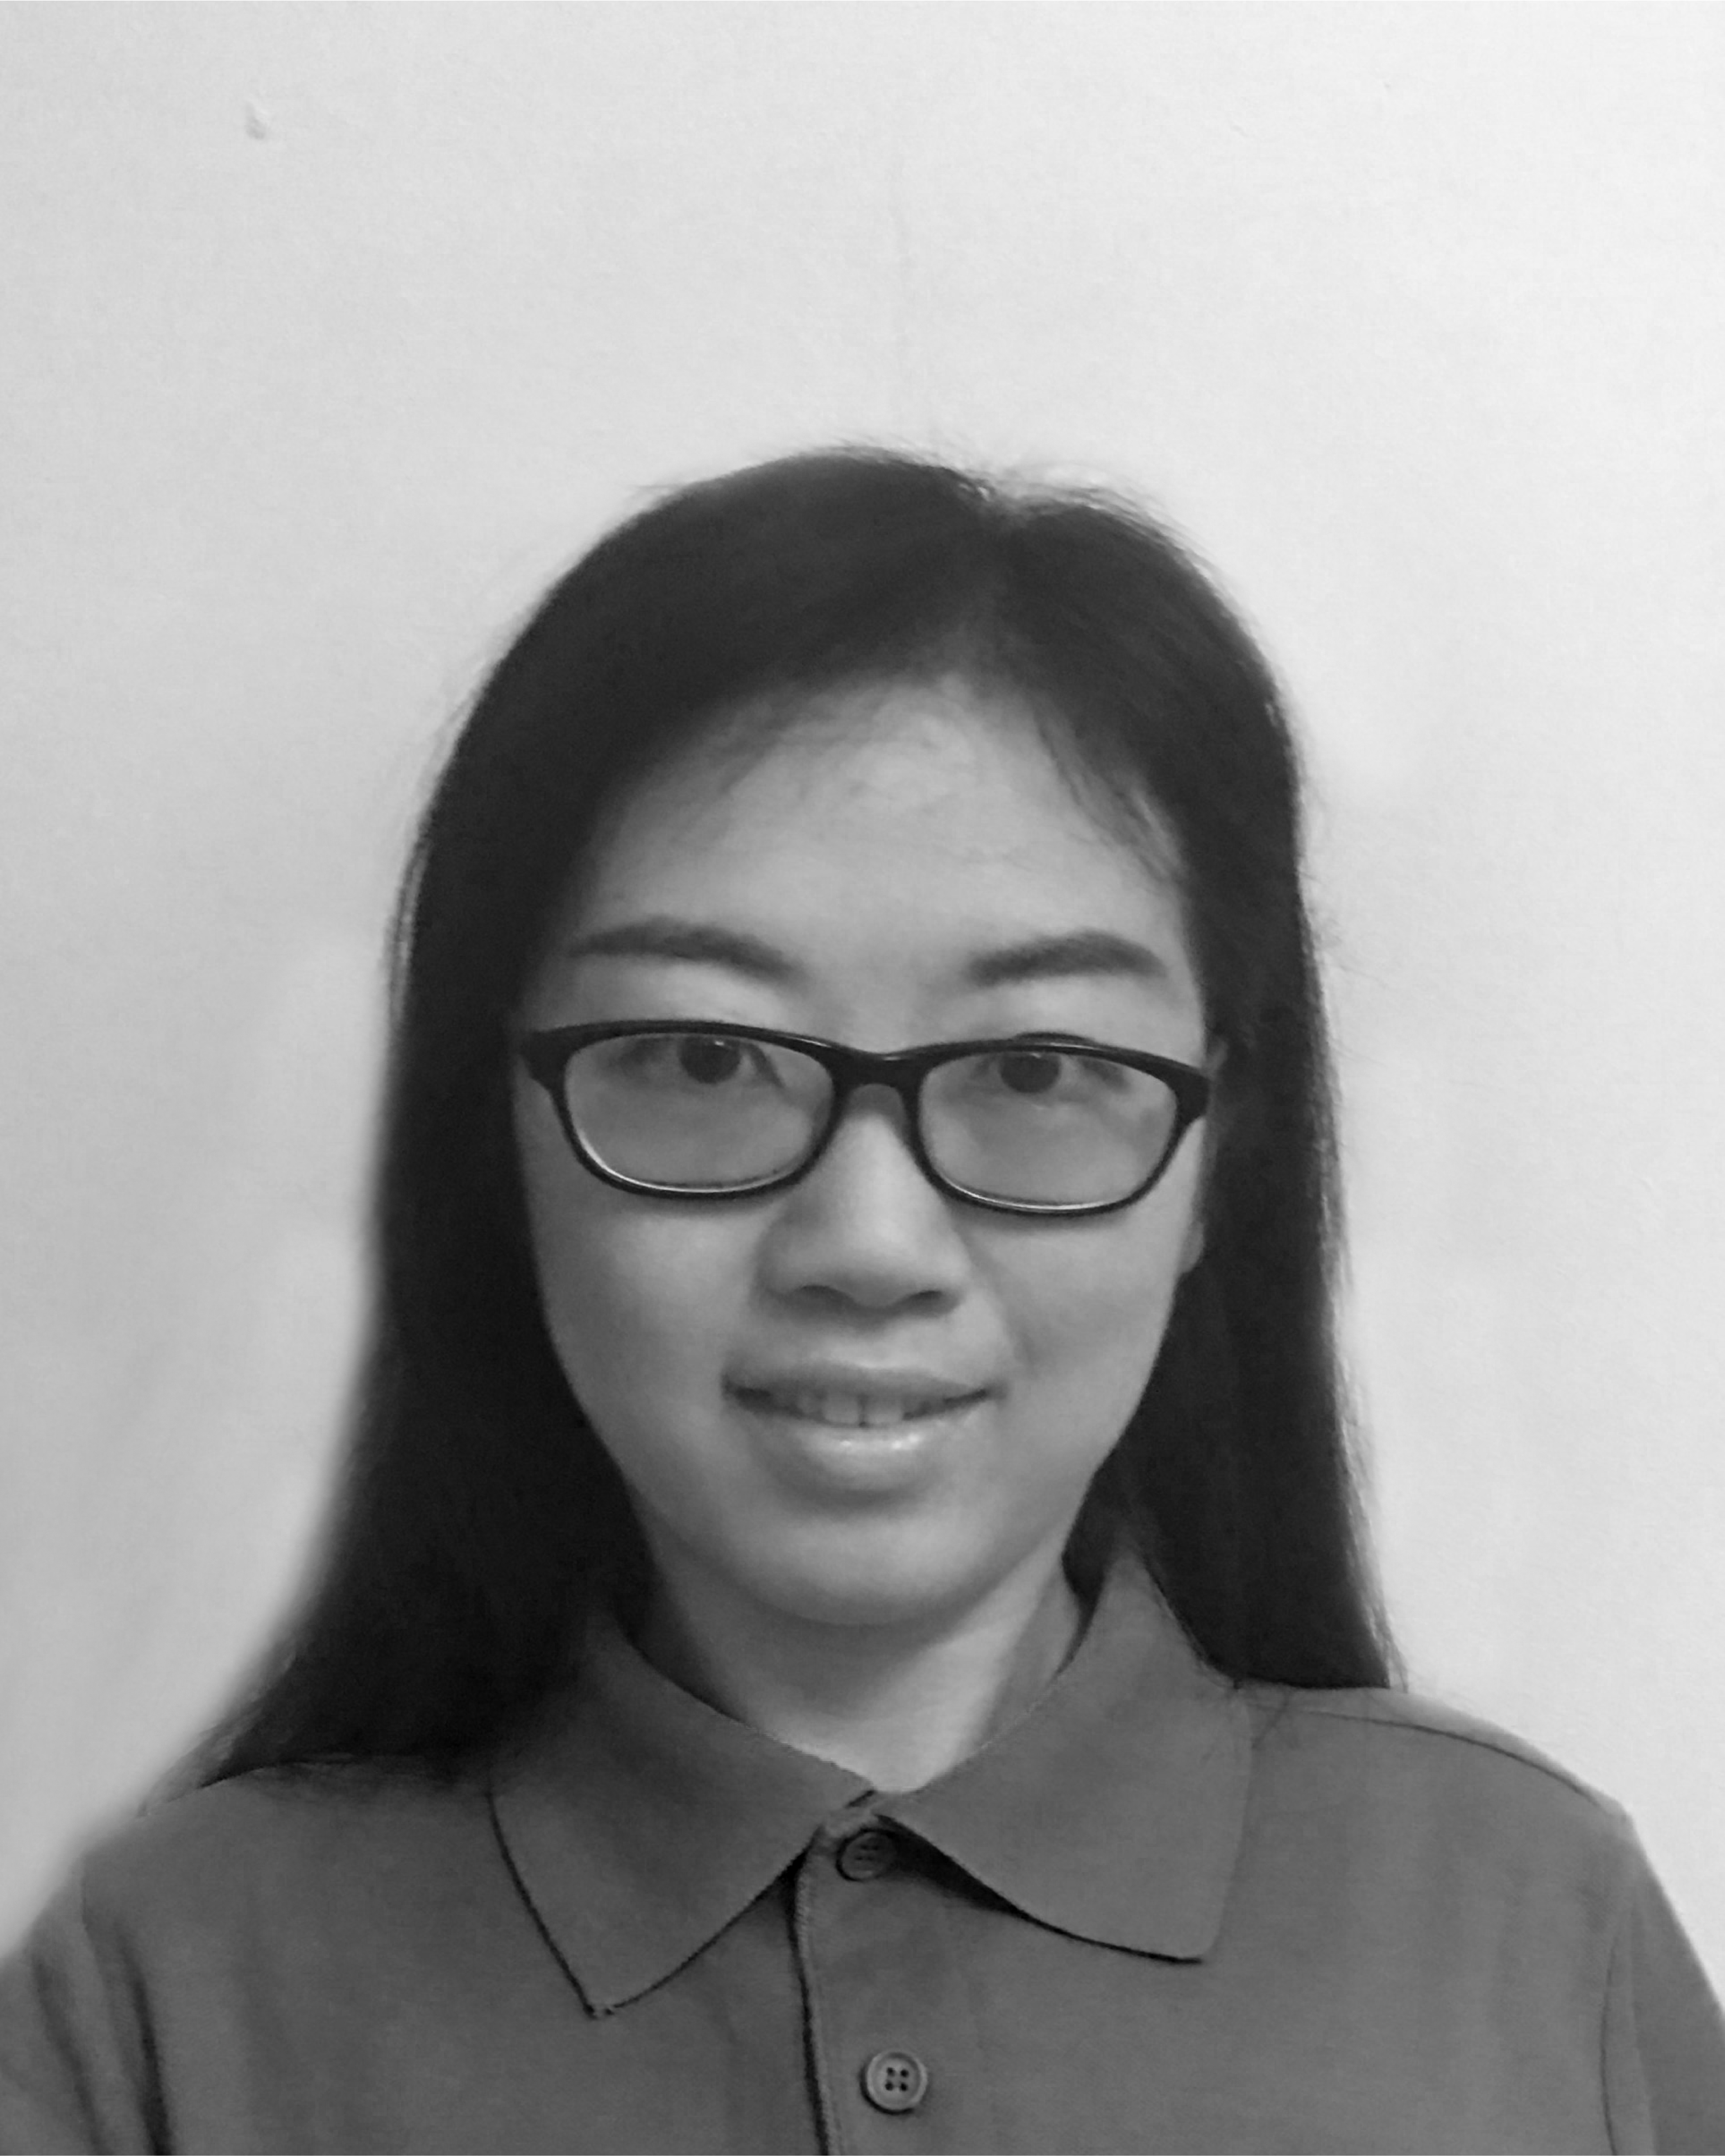
\includegraphics[width=1in,height=1.25in,clip,keepaspectratio]{bio/wq}}]{QI WANG} received the B.Eng. degree in information security from Wuhan University, China. She is currently working toward the Ph.D. degree in the State Key Laboratory of Information Engineering in Surveying, Mapping and Remote Sensing, Wuhan University. Her research interests include transport geographic information system, spatiotemporal data analysis, mining and visualization.
\end{IEEEbiography}

\begin{IEEEbiography}[{\includegraphics[width=1in,height=1.25in,clip,keepaspectratio]{bio/minlu}}]{Min lu} is an associate researcher at ShenZhen University. Her major research interest is data visualization and visual analytics, especially focusing on the urban data. She received Ph.D degree in Computer Science from Peking University in 2017 and BS degree in Computer Science from Beijing Normal University in 2011.
\end{IEEEbiography}

\begin{IEEEbiography}[{\includegraphics[width=1in,height=1.25in,clip,keepaspectratio]{bio/lqq}}]{Qingquan Li} received the Ph.D. degree in geographic information system (GIS) and photogrammetry from Wuhan Technical University of Surveying and Mapping, Wuhan, China, in 1998. He is currently a Professor with Shenzhen University, Guangdong, China, and Wuhan University, Wuhan, China. His research areas include 3-D and dynamic data modeling in GIS, location-based service, surveying engineering, integration of GIS, Global Positioning System and remote sensing, intelligent transportation system, and urban informatics.
\end{IEEEbiography}

\EOD

\end{document} 